% !TeX program = xelatex
\documentclass[a4paper,10pt]{article}

% ============================================================================
% សន្លឹកកិច្ចការសិស្ស ស-ខ្មៅ (Student Fill-In Worksheet — No-LCD Classroom)
% មេរៀនទី១៦ (១៦.២)៖ លក្ខណៈមេដ្យាទ័រនៃត្រីកោណ (ត្រូវគ្នា ១០០% នឹង LS_Plan_PBIS.tex)
% ============================================================================
\usepackage[a4paper, left=0.95cm, right=0.95cm, top=0.75cm, bottom=0.90cm, footskip=0.48cm]{geometry}
\usepackage{amsmath}
\usepackage{unicode-math}
\usepackage{fontspec}
\usepackage{array, colortbl}
\usepackage[table]{xcolor}
\usepackage{enumitem}
\usepackage{pifont}
\usepackage{fancyhdr}
\usepackage{lastpage}
\usepackage{tikz}
\usepackage[most]{tcolorbox}
\usetikzlibrary{calc, arrows.meta, angles, quotes, decorations.markings, babel}

\makeatletter
\let\@expl@@@mark@update@singlecol@structures@@\relax
\makeatother

% ============================================================================
% ការកំណត់ពុម្ពអក្សរ (Cross-Platform Font Resolver)
% ============================================================================
\providecommand{\NGSFindFonts}{%
  \IfFileExists{C:/Windows/Fonts/cambria.ttc}{%
    \def\NGSSysPath{C:/Windows/Fonts/}%
    \def\NGSUserPath{C:/Users/KIT/AppData/Local/Microsoft/Windows/Fonts/}%
  }{%
    \IfFileExists{./fonts/KhmerOSsiemreap.ttf}{\def\NGSSysPath{./fonts/}\def\NGSUserPath{./fonts/}}{%
    \IfFileExists{../fonts/KhmerOSsiemreap.ttf}{\def\NGSSysPath{../fonts/}\def\NGSUserPath{../fonts/}}{%
    \IfFileExists{../../fonts/KhmerOSsiemreap.ttf}{\def\NGSSysPath{../../fonts/}\def\NGSUserPath{../../fonts/}}{%
    \IfFileExists{../../../fonts/KhmerOSsiemreap.ttf}{\def\NGSSysPath{../../../fonts/}\def\NGSUserPath{../../../fonts/}}{%
    \IfFileExists{../../../../fonts/KhmerOSsiemreap.ttf}{\def\NGSSysPath{../../../../fonts/}\def\NGSUserPath{../../../../fonts/}}{%
    \IfFileExists{../../../../../fonts/KhmerOSsiemreap.ttf}{\def\NGSSysPath{../../../../../fonts/}\def\NGSUserPath{../../../../../fonts/}}{%
    \IfFileExists{../../../../../../fonts/KhmerOSsiemreap.ttf}{\def\NGSSysPath{../../../../../../fonts/}\def\NGSUserPath{../../../../../../fonts/}}{%
      \def\NGSSysPath{../../../../../../../fonts/}\def\NGSUserPath{../../../../../../../fonts/}%
    }}}}}}}%
  }%
}
\NGSFindFonts

\setmathfont[Path={\NGSSysPath}, FontIndex=1, Scale=1.02]{cambria.ttc}
\defaultfontfeatures{Ligatures=TeX}

\setmainfont[
  Path={\NGSUserPath},
  Extension=.ttf,
  Script=Khmer,
  BoldFont={KhmerOSsiemreap},
  BoldFeatures={FakeBold=1.8},
  ItalicFont={KhmerOSsiemreap},
  ItalicFeatures={FakeSlant=0.25},
  BoldItalicFont={KhmerOSsiemreap},
  BoldItalicFeatures={FakeBold=1.8, FakeSlant=0.25}
]{KhmerOSsiemreap}

\newfontfamily\muol[Path={\NGSUserPath}, Extension=.ttf, Script=Khmer]{KhmerOSmuollight}
\newfontfamily\TimesEn[Path={\NGSSysPath}, Extension=.ttf, BoldFont={timesbd}, ItalicFont={timesi}, BoldItalicFont={timesbi}]{times}

\XeTeXlinebreaklocale "km"
\XeTeXlinebreakskip = 0pt plus 1pt minus 0.1pt

\definecolor{panelgray}{gray}{0.93}
\definecolor{headgray}{gray}{0.85}

\pagestyle{fancy}
\fancyhf{}
\renewcommand{\headrulewidth}{0pt}
\fancyfoot[L]{\fontsize{8pt}{10pt}\selectfont អនុវិទ្យាល័យព្រះក្រសាំង \en{---} គណិតវិទ្យា ថ្នាក់ទី៨ \en{|} មេរៀនទី១៦ (១៦.២ លក្ខណៈមេដ្យាទ័រនៃត្រីកោណ)}
\fancyfoot[R]{\fontsize{8.2pt}{10pt}\selectfont ទំព័រ \en{\thepage\ / \pageref{LastPage}}}

\setlength{\parindent}{0pt}
\setlength{\parskip}{0pt}
\setlength{\tabcolsep}{4pt}

\newcommand{\en}[1]{{\TimesEn #1}}
\newcommand{\enbf}[1]{{\TimesEn\textbf{#1}}}
\newcommand{\unit}[1]{\,\text{\en{#1}}}
\newcommand{\cnum}[1]{\mbox{\fontsize{10pt}{12pt}\selectfont\ding{\numexpr181+#1\relax}}}
\newcommand{\chkbox}{\tikz[baseline=-0.15ex]\draw[black, line width=0.85pt] (0,0) rectangle (0.25cm,0.25cm);}
\newcommand{\blank}[1]{\makebox[#1]{\dotfill}}
\newcommand{\tri}[1]{\ensuremath{\triangle #1}}
\newcommand{\ang}[1]{\ensuremath{\angle #1}}
\newcommand{\cg}{\ensuremath{\cong}}

\newcommand{\rightbox}[4][0.18]{%
  \draw[black, line width=0.8pt]
    ($(#3)!#1!(#2)$) -- ($($(#3)!#1!(#2)$)+($(#3)!#1!(#4)$)-(#3)$) -- ($(#3)!#1!(#4)$);
}

\newcommand{\secbar}[2]{%
  \vspace{3pt}%
  \begin{tcolorbox}[
    enhanced, sharp corners, colback=headgray, colframe=black,
    boxrule=0.9pt, boxsep=1pt, top=2.5pt, bottom=2.5pt, left=6pt, right=6pt,
    after skip=3pt
  ]
    {\muol\fontsize{9.2pt}{13.5pt}\selectfont #1}\hfill{\fontsize{8.3pt}{11.5pt}\selectfont\textbf{#2}}
  \end{tcolorbox}%
}

\tikzset{
  tk1/.style={postaction={decorate},decoration={markings,mark=at position 0.50 with {\draw[black, line width=0.90pt](0,-0.095)--(0,0.095);}}},
  tk2/.style={postaction={decorate},decoration={markings,
    mark=at position 0.45 with {\draw[black, line width=0.90pt](0,-0.095)--(0,0.095);},
    mark=at position 0.55 with {\draw[black, line width=0.90pt](0,-0.095)--(0,0.095);}}},
  tk3/.style={postaction={decorate},decoration={markings,
    mark=at position 0.42 with {\draw[black, line width=0.90pt](0,-0.095)--(0,0.095);},
    mark=at position 0.50 with {\draw[black, line width=0.90pt](0,-0.095)--(0,0.095);},
    mark=at position 0.58 with {\draw[black, line width=0.90pt](0,-0.095)--(0,0.095);}}}
}

\newcolumntype{L}[1]{>{\raggedright\arraybackslash}p{#1}}
\newcolumntype{C}[1]{>{\centering\arraybackslash}p{#1}}

\begin{document}
\fontsize{9.4pt}{13.8pt}\selectfont

% ============================================================================
% ទំព័រទី ១៖ ក្បាលសន្លឹកកិច្ចការ + E1 + E2 (ករណីប្រៀបធៀបទាំង ៣ & ខ្សែសង្វាក់អំណះអំណាង) + E3
% ============================================================================
\begin{tcolorbox}[
  enhanced, sharp corners, colback=white, colframe=black,
  boxrule=1.1pt, boxsep=2pt, top=3pt, bottom=3pt, left=6pt, right=6pt, after skip=3pt
]
  \begin{center}
    {\muol\fontsize{10.5pt}{15pt}\selectfont សន្លឹកកិច្ចការសិស្ស \enbf{---} គណិតវិទ្យា ថ្នាក់ទី៨ \enbf{(}មេរៀនទី១៦ ៖ ១៦\enbf{.}២ លក្ខណៈមេដ្យាទ័រនៃត្រីកោណ\enbf{)}}\\[2pt]
    {\fontsize{8.8pt}{12pt}\selectfont
    ឈ្មោះសិស្ស / ដៃគូ៖ \blank{6.2cm} \hspace{0.2cm}
    ថ្នាក់៖ \blank{1.4cm} \hspace{0.2cm}
    ក្រុម៖ \blank{1.2cm} \hspace{0.2cm}
    កាលបរិច្ឆេទ៖ \blank{2.8cm}}
  \end{center}
\end{tcolorbox}

% --- E1 Engage ---
\begin{tcolorbox}[
  enhanced, sharp corners, colback=panelgray, colframe=black,
  boxrule=0.8pt, boxsep=1.5pt, top=2.5pt, bottom=2.5pt, left=6pt, right=6pt, after skip=3pt
]
  \textbf{បេសកកម្មទី១ (\en{E1 - Engage})៖ ទីតាំងអណ្ដូងទឹកស្អាតរួមសម្រាប់សាលារៀនភូមិទាំងបី}\\
  ឃុំមួយចង់ជីកអណ្ដូងទឹករួមតែមួយត្រង់ចំណុច $O$ ឱ្យមានចម្ងាយស្មើគ្នាពីសាលារៀនភូមិទាំងបី $A, B$ និង $C$ ($OA=OB=OC$) ។\\
  $\blacktriangleright$ \textbf{ទស្សន៍ទាយ (\en{Predict})៖} (១) រក $O$ តាម៖ \chkbox\ មេដ្យាន \hspace{0.2cm} \chkbox\ មេដ្យាទ័រ \hspace{0.4cm}
  (២) តើ $O$៖ \chkbox\ នៅក្នុងត្រីកោណជានិច្ច \hspace{0.2cm} \chkbox\ អាចនៅលើជ្រុង ឬនៅក្រៅត្រីកោណ
\end{tcolorbox}

% --- E2 Explore Part A: Contrasting Cases ---
\secbar{ផ្នែកទី១ \enbf{(}ក\enbf{)} ៖ ករណីប្រៀបធៀបទាំង ៣ \enbf{(Contrasting Cases)} ដោយអេគែរនិងដែកឈាន \enbf{(E2)}}{ការងារជាដៃគូ \en{6 min}}

ចំណុចកណ្ដាលជ្រុងនីមួយៗត្រូវបានដៅរួចហើយ និងមេដ្យាទ័រទី១ ត្រូវបានគូសជាគំរូ ។ ចូរប្រើ \textbf{អេគែរ} គូសមេដ្យាទ័រពីរទៀតរកចំណុចប្រសព្វ $O$ រួចប្រើ \textbf{ដែកឈាន} គូសរង្វង់ផ្ចិត $O$ កាំ $OA$ កាត់តាមកំពូលទាំងបី៖\\[3pt]
\noindent
{\renewcommand{\arraystretch}{1.25}
\begin{tabular}{|C{6.05cm}|C{6.05cm}|C{6.05cm}|}
  \hline
  \cellcolor{headgray}\textbf{ករណីទី១៖ ត្រីកោណមុំស្រួច $\tri{ABC}$} &
  \cellcolor{headgray}\textbf{ករណីទី២៖ ត្រីកោណកែង $\tri{DEF}$ ($\ang{D}=90^\circ$)} &
  \cellcolor{headgray}\textbf{ករណីទី៣៖ ត្រីកោណមុំទាល $\tri{MNP}$ ($\ang{M}>90^\circ$)} \\
  \hline
  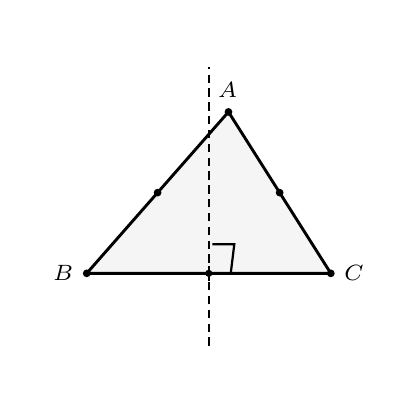
\begin{tikzpicture}[scale=1.00, baseline=(current bounding box.center), every node/.style={font=\footnotesize, text=black}]
    \path (-2.3,-1.48) rectangle (2.3,3.12);
    \coordinate (B) at (-1.55,0);
    \coordinate (C) at (1.55,0);
    \coordinate (A) at (0.25,2.05);
    \coordinate (M1) at ($(B)!0.5!(C)$);
    \coordinate (M2) at ($(A)!0.5!(C)$);
    \coordinate (M3) at ($(A)!0.5!(B)$);
    \fill[gray!8] (A) -- (B) -- (C) -- cycle;
    \draw[black, line width=1.05pt] (A) -- (B) -- (C) -- cycle;
    \draw[black, line width=0.85pt, densely dashed] (0,-0.92) -- (0,2.62);
    \rightbox[0.18]{A}{M1}{C}
    \draw[black, line width=0.8pt, tk1] (B) -- (M1) (M1) -- (C);
    \fill[black] (A) circle (1.4pt) node[above=1.5pt] {$A$};
    \fill[black] (B) circle (1.4pt) node[left=1.5pt] {$B$};
    \fill[black] (C) circle (1.4pt) node[right=1.5pt] {$C$};
    \fill[black] (M1) circle (1.3pt);
    \fill[black] (M2) circle (1.4pt);
    \fill[black] (M3) circle (1.4pt);
  \end{tikzpicture}
  &
  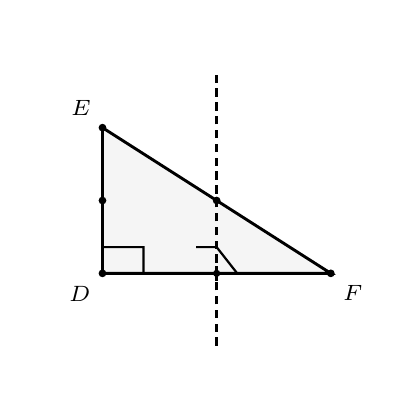
\begin{tikzpicture}[scale=1.00, baseline=(current bounding box.center), every node/.style={font=\footnotesize, text=black}]
    \path (-2.3,-1.48) rectangle (2.3,3.12);
    \coordinate (D) at (-1.35,0);
    \coordinate (F) at (1.55,0);
    \coordinate (E) at (-1.35,1.85);
    \coordinate (M1) at ($(D)!0.5!(F)$);
    \coordinate (M2) at ($(D)!0.5!(E)$);
    \coordinate (M3) at ($(E)!0.5!(F)$);
    \fill[gray!8] (D) -- (E) -- (F) -- cycle;
    \draw[black, line width=1.05pt] (D) -- (E) -- (F) -- cycle;
    \rightbox[0.18]{E}{D}{F}
    \draw[black, line width=0.85pt, densely dashed] (0.10,-0.92) -- (0.10,2.55);
    \rightbox[0.18]{E}{M1}{F}
    \draw[black, line width=0.8pt, tk1] (D) -- (M1) (M1) -- (F);
    \fill[black] (D) circle (1.4pt) node[below left=1pt] {$D$};
    \fill[black] (F) circle (1.4pt) node[below right=1pt] {$F$};
    \fill[black] (E) circle (1.4pt) node[above left=1pt] {$E$};
    \fill[black] (M1) circle (1.3pt);
    \fill[black] (M2) circle (1.4pt);
    \fill[black] (M3) circle (1.4pt);
  \end{tikzpicture}
  &
  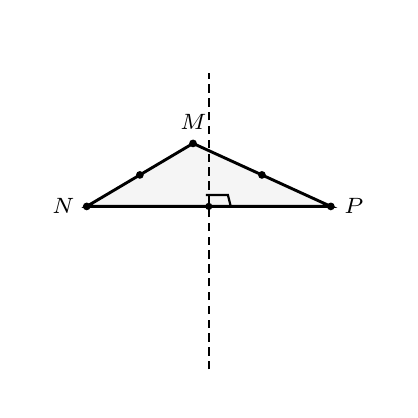
\begin{tikzpicture}[scale=1.00, baseline=(current bounding box.center), every node/.style={font=\footnotesize, text=black}]
    \path (-2.3,-1.48) rectangle (2.3,3.12);
    \coordinate (N) at (-1.55,0.85);
    \coordinate (P) at (1.55,0.85);
    \coordinate (M) at (-0.20,1.65);
    \coordinate (M1) at ($(N)!0.5!(P)$);
    \coordinate (M2) at ($(M)!0.5!(P)$);
    \coordinate (M3) at ($(M)!0.5!(N)$);
    \fill[gray!8] (M) -- (N) -- (P) -- cycle;
    \draw[black, line width=1.05pt] (M) -- (N) -- (P) -- cycle;
    \draw[black, line width=0.85pt, densely dashed] (0,-1.22) -- (0,2.55);
    \rightbox[0.18]{M}{M1}{P}
    \draw[black, line width=0.8pt, tk1] (N) -- (M1) (M1) -- (P);
    \fill[black] (M) circle (1.4pt) node[above=1.5pt] {$M$};
    \fill[black] (N) circle (1.4pt) node[left=1.5pt] {$N$};
    \fill[black] (P) circle (1.4pt) node[right=1.5pt] {$P$};
    \fill[black] (M1) circle (1.3pt);
    \fill[black] (M2) circle (1.4pt);
    \fill[black] (M3) circle (1.4pt);
  \end{tikzpicture} \\
  \hline
  ទីតាំង $O$៖ \chkbox\ ក្នុង \;\chkbox\ លើជ្រុង \;\chkbox\ ក្រៅ &
  ទីតាំង $O$៖ \chkbox\ ក្នុង \;\chkbox\ លើជ្រុង \;\chkbox\ ក្រៅ &
  ទីតាំង $O$៖ \chkbox\ ក្នុង \;\chkbox\ លើជ្រុង \;\chkbox\ ក្រៅ \\
  \hline
\end{tabular}}\\[5pt]
$\blacktriangleright$ \textbf{សង្កេតរួម៖} ពេលយកដែកឈានដាក់ផ្ចិតត្រង់ $O$ ហើយបើកកាំស្មើ $OA$ (ឬ $OD, OM$) តើរង្វង់កាត់តាមកំពូលពីរទៀតគ្រប់ករណីទាំង ៣ ដែរឬទេ? \hspace{0.2cm} \chkbox\ កាត់តាមទាំងអស់ \hspace{0.25cm} \chkbox\ មិនកាត់តាម

\vspace{6pt}
% --- E2 Explore Part B: Transitive Locus Flowchart ---
\secbar{ផ្នែកទី១ \enbf{(}ខ\enbf{)} ៖ ដ្យាក្រាមខ្សែសង្វាក់អំណះអំណាង \enbf{---} ឧទាហរណ៍ ទំព័រ ២០៧ \enbf{(Locus Chain)}}{ការងារជាដៃគូ \en{5 min}}

\noindent
\begin{minipage}[c]{12.2cm}
  ក្នុង $\tri{ABC}$ តាង $O$ ជាចំណុចប្រសព្វរវាងមេដ្យាទ័រ $d$ (នៃជ្រុង $AB$) និងមេដ្យាទ័រ $d_1$ (នៃជ្រុង $BC$) ។ ចូរបំពេញចន្លោះដើម្បីបង្ហាញថាមេដ្យាទ័រទីបី $d_2$ (នៃជ្រុង $AC$) ក៏កាត់តាម $O$ ដែរ៖\\[3.5pt]
  $1.$ ដោយ $O \in d$ (មេដ្យាទ័រនៃអង្កត់ $AB$) $\Longrightarrow OA = \blank{1.3cm} \quad (1)$\\[3.5pt]
  $2.$ ដោយ $O \in d_1$ (មេដ្យាទ័រនៃអង្កត់ $BC$) $\Longrightarrow OB = \blank{1.3cm} \quad (2)$\\[3.5pt]
  $3.$ តាម $(1)$ និង $(2)$ គេទាញបានសមភាពបន្ត៖ $OA = OB = \blank{1.3cm}$ ជាពិសេស $OA = \blank{1.3cm}$ ។\\[3.5pt]
  $4.$ ហេតុនេះ $O$ ស្ថិតនៅស្មើចម្ងាយពី $A$ និង $C$ $\Longrightarrow O$ ស្ថិតនៅលើ \blank{2.3cm} $d_2$ នៃអង្កត់ $AC$ ។\\[3.5pt]
  $5.$ ដូចនេះ មេដ្យាទ័រទាំងបី $d, d_1, d_2$ ប្រសព្វគ្នាត្រង់ចំណុច \blank{0.9cm} តែមួយគត់ ហើយរង្វង់ផ្ចិត $O$ កាំ $OA$ កាត់តាមកំពូលទាំងបី $A, B, C$ ហៅថា \textbf{រង្វង់\blank{3.2cm}} ។
\end{minipage}%
\hfill
\begin{minipage}[c]{6.5cm}
  \centering
  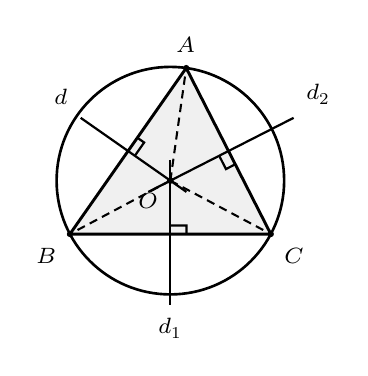
\begin{tikzpicture}[scale=0.86, every node/.style={font=\footnotesize, text=black}]
    \coordinate (O) at (0,0);
    \def\R{1.68}
    \coordinate (A) at (82:\R);
    \coordinate (B) at (208:\R);
    \coordinate (C) at (-28:\R);
    \coordinate (K) at ($(A)!0.5!(B)$);
    \coordinate (M) at ($(B)!0.5!(C)$);
    \coordinate (N) at ($(A)!0.5!(C)$);
    \draw[black, line width=0.95pt] (O) circle (\R);
    \fill[gray!12] (A) -- (B) -- (C) -- cycle;
    \draw[black, line width=1.05pt] (A) -- (B) -- (C) -- cycle;
    \draw[black, line width=0.8pt] ($(O)!-0.38!(K)$) -- ($(O)!2.12!(K)$) node[above left=1pt] {$d$};
    \draw[black, line width=0.8pt] ($(O)!-0.38!(M)$) -- ($(O)!2.32!(M)$) node[below=1pt] {$d_1$};
    \draw[black, line width=0.8pt] ($(O)!-0.38!(N)$) -- ($(O)!2.12!(N)$) node[above right=1pt] {$d_2$};
    \rightbox[0.16]{O}{K}{A}
    \rightbox[0.16]{O}{M}{C}
    \rightbox[0.16]{O}{N}{C}
    \draw[black, line width=0.75pt, densely dashed] (O) -- (A) (O) -- (B) (O) -- (C);
    \fill[black] (A) circle (1.3pt) node[above=2pt] {$A$};
    \fill[black] (B) circle (1.3pt) node[below left=1.5pt] {$B$};
    \fill[black] (C) circle (1.3pt) node[below right=1.5pt] {$C$};
    \fill[black] (O) circle (1.4pt) node[below left=1pt] {$O$};
  \end{tikzpicture}
\end{minipage}

\vspace{6pt}
% --- E3 Explain: Theorem & Warrant Bank ---
\secbar{ផ្នែកទី២ ៖ បញ្ញត្តិទ្រឹស្តីបទ និងធនាគារហេតុផល \enbf{(E3 - Explain)}}{សង្ខេបរួមគ្នា \en{6 min}}

\begin{tcolorbox}[
  enhanced, sharp corners, colback=white, colframe=black,
  boxrule=0.9pt, boxsep=2.8pt, top=4pt, bottom=4pt, left=6pt, right=6pt
]
  $\bullet$ \textbf{ទ្រឹស្តីបទ (ទំ.២០៧)៖} មេដ្យាទ័រទាំងបីនៃត្រីកោណមួយប្រសព្វគ្នាត្រង់ចំណុចតែមួយ ដែលឋិតនៅ \textbf{\blank{3.6cm}} ពីកំពូលទាំងបីនៃត្រីកោណនោះ ($OA=OB=OC$) ។ ចំណុចនេះជា \textbf{ផ្ចិត\blank{3.8cm}} ។\\[3.5pt]
  $\bullet$ \textbf{សង្ខេបទីតាំងផ្ចិត $O$៖} ត្រីកោណមុំស្រួច $\to$ នៅក្នុង \;\textbar\; ត្រីកោណកែង $\to$ ចំកណ្ដាល\blank{2.2cm} \;\textbar\; ត្រីកោណមុំទាល $\to$ នៅ\blank{1.5cm} ។\\[3.5pt]
  $\bullet$ \textbf{ធនាគារហេតុផល៖}
  \cnum{1} និយមន័យមេដ្យាទ័រ \;\textbar\;
  \cnum{2} $M\in d \Leftrightarrow MA=MB$ \;\textbar\;
  \cnum{3} ផ្ចិតរង្វង់ចារឹកក្រៅ ($OA=OB=OC$) \;\textbar\;
  \cnum{4} មេដ្យានទៅអ៊ីប៉ូតេនុស ($OM=\frac{AB}{2}$) \;\textbar\;
  \cnum{5} ករណី អ.ជ / ជ្រុងឈមប្រលេឡូក្រាម
\end{tcolorbox}

\newpage

% ============================================================================
% ទំព័រទី ២៖ E4 (លំហាត់គំរូ + ប្រតិបត្តិ) + E5 (វិនិច្ឆ័យខុស-ត្រូវ & Exit Check) + កិច្ចការផ្ទះ
% ============================================================================

\secbar{ផ្នែកទី៣ ៖ ពង្រីកចំណេះដឹង \enbf{---} លំហាត់គំរូ និងប្រតិបត្តិសៀវភៅគោល \enbf{(E4 - Elaborate)}}{អនុវត្ត \en{10 min}}

\noindent
\begin{minipage}[t]{9.4cm}\vspace{0pt}
  \begin{tcolorbox}[
    enhanced, sharp corners, colback=white, colframe=black, equal height group=rowE4,
    boxrule=0.85pt, boxsep=2.2pt, top=3.5pt, bottom=3.5pt, left=5pt, right=5pt
  ]
    \textbf{៣.ក លំហាត់គំរូ (ទំ.២០៧\,\en{--}\,២០៨)៖}\\
    $\tri{AMB}$ ជាត្រីកោណកែងត្រង់ $M$ ហើយ $O$ ជាចំណុចកណ្ដាលនៃអង្កត់ $AB$ ។ តាម $O$ គេគូសបន្ទាត់កែងនឹង $AM$ ត្រង់ $N$ ។ បង្ហាញថា $ON$ ជាមេដ្យាទ័រនៃអង្កត់ $AM$ ៖
    \begin{center}
      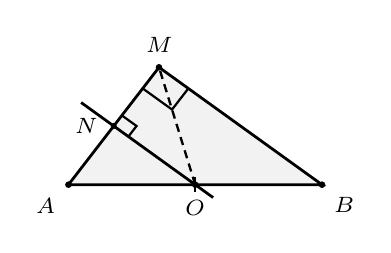
\begin{tikzpicture}[scale=0.92, every node/.style={font=\footnotesize, text=black}]
        \coordinate (A) at (-1.75,0);
        \coordinate (B) at (1.75,0);
        \coordinate (O) at (0,0);
        \coordinate (M) at (-0.50,1.62);
        \coordinate (N) at ($(A)!0.5!(M)$);
        \fill[gray!10] (A) -- (M) -- (B) -- cycle;
        \draw[black, line width=1.0pt] (A) -- (M) -- (B) -- cycle;
        \draw[black, line width=0.85pt, densely dashed] (O) -- (M);
        \draw[black, line width=1.0pt] ($(O)!-0.22!(N)$) -- ($(O)!1.40!(N)$);
        \rightbox[0.18]{A}{M}{B}
        \rightbox[0.18]{O}{N}{M}
        \draw[black, line width=0.8pt, tk1] (A) -- (O) (O) -- (B);
        \fill[black] (A) circle (1.3pt) node[below left=1pt] {$A$};
        \fill[black] (B) circle (1.3pt) node[below right=1pt] {$B$};
        \fill[black] (O) circle (1.3pt) node[below=2pt] {$O$};
        \fill[black] (M) circle (1.3pt) node[above=2pt] {$M$};
        \fill[black] (N) circle (1.2pt) node[left=3pt] {$N$};
      \end{tikzpicture}
    \end{center}
    \vspace{-3pt}
    -- ក្នុងត្រីកោណកែង $\tri{AMB}$ មាន $O$ កណ្ដាលអ៊ីប៉ូតេនុស $AB$ នោះ $OM$ ជាមេដ្យាន $\Rightarrow OM = OA = \dfrac{\blank{0.8cm}}{2}$ (ហេតុផល \blank{0.8cm}) ។\\[1.5pt]
    -- ក្នុងត្រីកោណកែង $\tri{ANO}$ និង $\tri{MNO}$ មាន៖\\
    \hspace*{0.3cm}អ៊ីប៉ូតេនុស $OA = \blank{1.0cm}$ និងជ្រុងកែង \blank{1.0cm} ជាជ្រុងរួម\\
    \hspace*{0.3cm}$\Rightarrow \tri{ANO} \cg \tri{MNO}$ តាមករណី \blank{1.2cm} (ហេតុផល \blank{0.8cm}) ។\\[1.5pt]
    -- ទាញបាន $NA = \blank{1.0cm}$ តែ $ON \perp AM \Rightarrow ON$ ជា \blank{1.9cm} នៃ $AM$ ។\\[2pt]
    $\blacktriangleright$ \textbf{ឆ្លុះបញ្ចាំង (\en{Looking-Back})៖} ដោយ $ON\perp AM$ និង $BM\perp AM$ នោះ $ON \parallel \blank{1.0cm}$ ហើយ $O$ កណ្ដាល $AB \Rightarrow N$ ជាកណ្ដាល $AM$!
  \end{tcolorbox}
\end{minipage}%
\hfill
\begin{minipage}[t]{9.4cm}\vspace{0pt}
  \begin{tcolorbox}[
    enhanced, sharp corners, colback=white, colframe=black, equal height group=rowE4,
    boxrule=0.85pt, boxsep=2.2pt, top=3.5pt, bottom=3.5pt, left=5pt, right=5pt
  ]
    \textbf{៣.ខ ប្រតិបត្តិ (ទំ.២០៨)៖ ស្ពានឆ្ពោះទៅកម្ពស់ត្រីកោណ}\\
    ក្នុង $\tri{ABC}$ គេគូសបន្ទាត់ $\Delta, \Delta', \Delta''$ កាត់តាម $A, B, C$ ហើយស្របនឹងជ្រុងឈមរៀងគ្នា បង្កើតបាន $\tri{A'B'C'}$ ។ តាង $H$ ជាជើងកម្ពស់គូសពី $A$ នៃ $\tri{ABC}$ ។ បង្ហាញថា $AH$ ជាមេដ្យាទ័រនៃ $B'C'$ ៖
    \begin{center}
      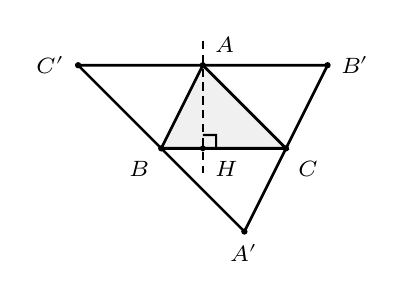
\begin{tikzpicture}[scale=0.88, every node/.style={font=\footnotesize, text=black}]
        \coordinate (B) at (-0.85,0.55);
        \coordinate (C) at (0.95,0.55);
        \coordinate (A) at (-0.25,1.75);
        \coordinate (Bp) at (1.55,1.75);
        \coordinate (Cp) at (-2.05,1.75);
        \coordinate (Ap) at (0.35,-0.65);
        \coordinate (H) at (-0.25,0.55);
        \fill[gray!12] (A) -- (B) -- (C) -- cycle;
        \draw[black, line width=0.95pt] (Cp) -- (Bp) -- (Ap) -- cycle;
        \draw[black, line width=1.0pt] (A) -- (B) -- (C) -- cycle;
        \draw[black, line width=0.95pt, densely dashed] (-0.25,2.10) -- (-0.25,0.20);
        \rightbox[0.16]{A}{H}{C}
        \fill[black] (A) circle (1.3pt) node[above right=1pt] {$A$};
        \fill[black] (B) circle (1.3pt) node[below left=1pt] {$B$};
        \fill[black] (C) circle (1.3pt) node[below right=1pt] {$C$};
        \fill[black] (H) circle (1.2pt) node[below right=1pt] {$H$};
        \fill[black] (Bp) circle (1.3pt) node[right=1.5pt] {$B'$};
        \fill[black] (Cp) circle (1.3pt) node[left=1.5pt] {$C'$};
        \fill[black] (Ap) circle (1.3pt) node[below=1pt] {$A'$};
      \end{tikzpicture}
    \end{center}
    \vspace{-3pt}
    $1.$ ចតុកោណ $ABCB'$ មាន $AB'\parallel BC$ និង $BB'\parallel AC$ នាំឱ្យវាជា \blank{2.4cm} $\Rightarrow AB' = \blank{1.0cm}$ ។\\[2pt]
    $2.$ ដូចគ្នាដែរ ចតុកោណ $AC'BC$ ជាប្រលេឡូក្រាម $\Rightarrow C'A = \blank{1.0cm}$ ។ ហេតុនេះ $C'A = AB'$ ពោលគឺ $A$ ជា \blank{2.2cm} នៃ $B'C'$ ។\\[2pt]
    $3.$ ដោយ $AH \perp BC$ ហើយបន្ទាត់ $B'C' \parallel \blank{1.0cm}$ គេបាន $AH \perp \blank{1.1cm}$ ត្រង់ $A$ ។ ដូចនេះ $AH$ ជា \blank{2.1cm} នៃ $B'C'$ ។
  \end{tcolorbox}
\end{minipage}

\vspace{2pt}
% --- E5 Evaluate: True/False Diagnosis + Exit Check ---
\secbar{ផ្នែកទី៤ ៖ វាយតម្លៃលទ្ធផលសិក្សា \enbf{---} វិនិច្ឆ័យខុស\enbf{-}ត្រូវ គណនា និងសំណួរត្រួតពិនិត្យរហ័ស \enbf{(E5)}}{ធ្វើដោយឯករាជ្យ \en{10 min}}

\noindent
\begin{minipage}[t]{10.2cm}\vspace{0pt}
  \begin{tcolorbox}[
    enhanced, sharp corners, colback=white, colframe=black, equal height group=rowE5,
    boxrule=0.85pt, boxsep=2.2pt, top=3.5pt, bottom=3.5pt, left=5pt, right=5pt
  ]
    \textbf{៤.ក វិនិច្ឆ័យខុស-ត្រូវដោយហេតុផល និងគណនា៖}\\[3pt]
    $1.$ «មេដ្យាទ័រនៃជ្រុងមួយរបស់ត្រីកោណ ត្រូវតែកាត់តាមកំពូលឈមជានិច្ច ។»\\
    \hspace*{0.2cm}\chkbox\ ត្រូវ \hspace{0.25cm} \chkbox\ ខុស \;\textbar\; ព្រោះ៖ \blank{5.7cm}\\[3.5pt]
    $2.$ «ផ្ចិតរង្វង់ចារឹកក្រៅ $O$ ស្ថិតនៅខាងក្នុងត្រីកោណជានិច្ច គ្រប់ប្រភេទត្រីកោណ ។»\\
    \hspace*{0.2cm}\chkbox\ ត្រូវ \hspace{0.25cm} \chkbox\ ខុស \;\textbar\; ព្រោះ៖ \blank{5.7cm}\\[3.5pt]
    $3.$ «បើ $\tri{ABC}$ កែងត្រង់ $A$ មានអ៊ីប៉ូតេនុស $BC = 10\unit{cm}$ នោះកាំរង្វង់ចារឹកក្រៅត្រីកោណនេះគឺ $R = 5\unit{cm}$ ។»\\
    \hspace*{0.2cm}\chkbox\ ត្រូវ \hspace{0.25cm} \chkbox\ ខុស \;\textbar\; ព្រោះ៖ \blank{5.7cm}\\[3.5pt]
    $4.$ \textbf{គណនា៖} $\tri{DEF}$ កែងត្រង់ $D$ មាន $DE=6\unit{cm}, DF=8\unit{cm}$ ។ តាមពីតាករ $EF = \blank{1.5cm}$ នាំឱ្យចម្ងាយពីផ្ចិតរង្វង់ចារឹកក្រៅ $O$ ទៅកំពូលទាំងបីគឺ $OD=OE=OF=\blank{1.5cm}$ ។
  \end{tcolorbox}
\end{minipage}%
\hfill
\begin{minipage}[t]{8.6cm}\vspace{0pt}
  \begin{tcolorbox}[
    enhanced, sharp corners, colback=white, colframe=black, equal height group=rowE5,
    boxrule=0.85pt, boxsep=2.2pt, top=3.5pt, bottom=3.5pt, left=5pt, right=5pt
  ]
    \textbf{៤.ខ សំណួរត្រួតពិនិត្យរហ័ស (\en{Exit Check})៖}\\
    ចូរគូសវង់ជុំវិញអក្សរនៃចម្លើយត្រឹមត្រូវតែមួយគត់៖\\[3.5pt]
    \textbf{សំណួរទី១៖} តាង $O$ ជាចំណុចប្រសព្វមេដ្យាទ័រទាំងបីនៃ $\tri{ABC}$ ។ បើ $OA = 6\unit{cm}$ តើប្រវែង $OB$ និង $OC$ ស្មើប៉ុន្មាន?\\
    \hspace*{0.15cm}\textbf{ក.} $OB=3\unit{cm},\, OC=3\unit{cm}$ \hspace{0.18cm}
    \textbf{ខ.} $OB=6\unit{cm},\, OC=6\unit{cm}$\\
    \hspace*{0.15cm}\textbf{គ.} $OB=4\unit{cm},\, OC=2\unit{cm}$ \hspace{0.18cm}
    \textbf{ឃ.} មិនអាចកំណត់បាន\\[5pt]
    \textbf{សំណួរទី២៖} ចំពោះត្រីកោណកែង តើផ្ចិតរង្វង់ចារឹកក្រៅ $O$ ស្ថិតនៅត្រង់ណា?\\
    \hspace*{0.15cm}\textbf{ក.} កំពូលមុំកែង \hspace{1.45cm}
    \textbf{ខ.} ខាងក្រៅត្រីកោណ\\
    \hspace*{0.15cm}\textbf{គ.} ចំណុចកណ្ដាលអ៊ីប៉ូតេនុស \hspace{0.2cm}
    \textbf{ឃ.} ទីប្រជុំទម្ងន់ $G$\\[4pt]
    \textbf{សំណួរទី៣ (បេសកកម្ម E1)៖} បើសាលារៀនភូមិទាំងបី $A,B,C$ បង្កើតបានជាត្រីកោណមុំទាល តើអណ្ដូងទឹករួម $O$ ស្ថិតនៅត្រង់ណា?\\
    \hspace*{0.15cm}\textbf{ក.} ខាងក្នុងត្រីកោណ \hspace{0.6cm} \textbf{ខ.} ខាងក្រៅត្រីកោណ
  \end{tcolorbox}
\end{minipage}

\vspace{2pt}
% --- Step 5 Homework Box ---
\secbar{ផ្នែកទី៥ ៖ កិច្ចការផ្ទះ និងការរៀបចំមេរៀនបន្ទាប់ \enbf{(}សៀវភៅគោល ទំព័រ ២០៨ និង ២១៣\enbf{)}}{ធ្វើនៅផ្ទះក្នុងសៀវភៅសរសេរ}

\begin{tcolorbox}[
  enhanced, sharp corners, colback=panelgray, colframe=black,
  boxrule=0.85pt, boxsep=2.5pt, top=3.5pt, bottom=3.5pt, left=6pt, right=6pt
]
  $1.$ \textbf{សរសេរសម្រាយពេញលេញនៃប្រតិបត្តិ (ទំ.២០៨)៖} សរសេរសម្រាយបំភ្លឺឡើងវិញឱ្យបានក្បោះក្បាយក្នុងសៀវភៅសរសេរថា បន្ទាត់កម្ពស់ $AH$ នៃ $\tri{ABC}$ គឺជាមេដ្យាទ័រនៃអង្កត់ $B'C'$ របស់ $\tri{A'B'C'}$ ។\\[3pt]
  $2.$ \textbf{លំហាត់ទី២ (ទំ.២១៣)៖} $ABCD$ ជាប្រលេឡូក្រាម, $I$ ជាចំណុចកណ្ដាលនៃអង្កត់ $AB$ និង $J$ ជាចំណុចកណ្ដាលនៃអង្កត់ $BC$ ។ ស្រាយបំភ្លឺថាបន្ទាត់ $AJ$ និង $CI$ ជួបគ្នានៅលើអង្កត់ទ្រូង $BD$ នៃប្រលេឡូក្រាម ។ \textit{(តម្រុយ៖ ពិនិត្យទីប្រជុំទម្ងន់នៃ $\tri{ABC}$ ។)}\\[3pt]
  $3.$ \textbf{កិច្ចការអានជាមុន៖} អានចំណុច \textbf{១៦.៣ លក្ខណៈកម្ពស់នៃត្រីកោណ} (សៀវភៅគោល ទំព័រ ២០៨\,\en{--}\,២១០) និងយកអេគែរមកគ្រប់គ្នា ។
\end{tcolorbox}

\end{document}
